

\documentclass[a4paper,12pt]{article}

\usepackage[T2A]{fontenc}
\usepackage[utf8]{inputenc}
\usepackage[english,russian]{babel}


\usepackage{array}

\usepackage{csquotes}



\usepackage{longtable}

\usepackage{graphicx}
\usepackage{float}%"Плавающие" картинки
\usepackage{wrapfig}%Обтекание фигур (таблиц, картинок и прочего)
\graphicspath{{images/}}
\usepackage[usenames]{color}


\usepackage{tikz}
\usepackage{pgfplots}

\usepackage[
bookmarks=true, colorlinks=true, unicode=true,
urlcolor=black,linkcolor=black, anchorcolor=black,
citecolor=black, menucolor=black, filecolor=black,
]{hyperref}

\usepackage{color}
\usepackage{caption}
\DeclareCaptionFont{white}{\color{black}}
\DeclareCaptionFormat{listing}{\colorbox{white}{\parbox{\textwidth}{#1#2#3}}}
\captionsetup[lstlisting]{format=listing,labelfont=white,textfont=white}

\usepackage{amsmath,amsfonts,amssymb,amsthm,mathtools} 
\usepackage{wasysym}

%\usepackage[cache=false]{minted}
\usepackage{cmap}
\usepackage{indentfirst}

\usepackage{listings} 
\usepackage{fancyvrb}

\usepackage{geometry}
\geometry{left=2cm}
\geometry{right=1.5cm}
\geometry{top=1cm}
\geometry{bottom=2cm}

\setlength{\parindent}{5ex}
\setlength{\parskip}{0.5em}

\newenvironment{comment}{}{}

\begin{document}
\lstset{ %
	language=C++,                 % выбор языка для подсветки (здесь это С)
	basicstyle=\small\sffamily, % размер и начертание шрифта для подсветки кода
	numbers=left,               % где поставить нумерацию строк (слева\справа)
	numberstyle=\tiny,           % размер шрифта для номеров строк
	stepnumber=1,                   % размер шага между двумя номерами строк
	numbersep=5pt,                % как далеко отстоят номера строк от подсвечиваемого кода
	backgroundcolor=\color{white}, % цвет фона подсветки - используем \usepackage{color}
	showspaces=false,            % показывать или нет пробелы специальными отступами
	showstringspaces=false,      % показывать или нет пробелы в строках
	showtabs=false,             % показывать или нет табуляцию в строках
	frame=single,              % рисовать рамку вокруг кода
	tabsize=2,                 % размер табуляции по умолчанию равен 2 пробелам
	captionpos=t,              % позиция заголовка вверху [t] или внизу [b] 
	breaklines=true,           % автоматически переносить строки (да\нет)
	breakatwhitespace=false, % переносить строки только если есть пробел
	escapeinside={\%*}{*)}   % если нужно добавить комментарии в коде
}


\begin{filecontents}{Vinograddd.dat}
	1 30350926
	2 30350926
	4 30350926
	8 30350926
	16 30350926
	32 30350926
\end{filecontents}

\begin{filecontents}{Thread_vinograddd.dat}
	1 31278636
	2 13545137
	4 10040994
	8 8486562
	16 8785022
	32 8936443
\end{filecontents}



% Титульный лист
\large
\begin{center}
	Федеральное государственное бюджетное образовательное учреждение 
	высшего образования <<Московский государственный технический 
	университет имени Н. Э. Баумана>> 
	(национальный исследовательский университет)
\end{center}

\vspace*{30mm} 

\huge
\begin{center}
	Дисциплина: <<Анализ алгоритмов>>
	
	Отчет по лабораторной работе №4
\end{center}

\vspace*{30mm} 

\huge
\begin{center}
	Тема работы:\\
	<<Многопоточность на примере умножения матриц>>
\end{center}
\vspace*{30mm} 

\large
\begin{flushright}
	Студент: Левушкин И. К. \\
	Группа: ИУ7-52Б \\
	Преподаватели: Волкова Л. Л., \\ Строганов Ю. В. \\
\end{flushright}

\vspace*{40mm}
\begin{center}
	Москва, 2019 г.  
\end{center}
\thispagestyle{empty}

\tableofcontents


\section*{Введение}
\addcontentsline{toc}{section}{Введение}

Алгоритм умножения матриц применяется во многих 
серьезных вычислительных задачах. Поиск способа 
оптимизации такой операции является довольно
важным вопросом.

\textbf{Цель лабораторной работы:} изучение метода динамического программирования на материале оптимизированного алгоритма Винограда и реализация многопоточности для него.

\textbf{Задачи работы:}
\begin{enumerate} 
	\item[1)] изучить алгоритм умножения матриц по Винограду;
	\item[2)] оптимизировать алгоритм Винограда;
	\item[3)] реализовать многопоточность для оптимизированного алгоритма Винограда;
	\item[3)] применить метод динамического программирования для реализации указанных алгоритмов;
	\item[4)] провести сравнительный анализ по затрачиваемому времени при разном количестве рабочих потоков;
	\item[5)] описать и обосновать полученные результаты в отчете, выполненного как расчётно-пояснительная записка к работе. 
\end{enumerate} 
\pagebreak


\section{Аналитический раздел}

В данном разделе анализируются классический подход
к решению задачи об умножении матриц, а также
алгоритм Винограда. 

\subsection{Описание алгоритмов}

\subsubsection{Классический алгоритм умножения матриц}

Матрица определяется как математический объект, 
записываемый в виде 
прямоугольной таблицы чисел, которая представляет 
собой совокупность строк 
и столбцов, на пересечении которых находятся ее 
элементы. Количество строк и столбцов является 
размерностью матрицы.

Пусть даны две матрицы $\mathbf{A}$ размерностью
$m \times q$ и $\mathbf{B}$ размерностью $q \times n$. 

Тогда результатом умножения матрицы $A$ на $B$
является матрица $\mathbf{C}$ размерностью $m \times n$,
в которой элемент $c_{ij}$ вычисляется 
следующим образом:

\[
c_{ij} = \sum_{k=1}^q a_{ik} \cdot b_{kj},
\]

\begin{flushleft}
	где \\
	$i = \overline{1, m},$ \\
	$j = \overline{1, n}.$
\end{flushleft}

Заметим, что операция умножения двух матриц возможна 
только в том случае, если число столбцов в первом сомножителе равно числу строк во втором.

\subsubsection{Умножение матриц по Винограду}

Если посмотреть на результат умножения двух матриц, то видно, что каждый элемент в нем представляет собой скалярное произведение соответствующих строки и столбца исходных матриц. Можно заметить также, что такое умножение допускает предварительную обработку, позволяющую часть работы выполнить заранее
~\cite{mcconell}.

Рассмотрим два вектора $\mathbf{V} = (v_1, v_2, v_3, v_4)$
и $\mathbf{W} = (w_1, w_2, w_3, w_4)$. Их скалярное 
произведение равно:

\[
\mathbf{V} \cdot \mathbf{W} = v_1 w_1 + v_2 w_2 
+ v_3 w_3 + v_4 w_4.
\]

Это равенство можно переписать в виде:

\begin{multline}
	\mathbf{V} \cdot \mathbf{W} = (v_1 + w_2) (v_2 + w_1) 
	+ (v_3 + w_4) (v_4 + w_3) \\
	- v_1 v_2 - v_3 v_4 
	- w_1 w_2 - w_3 w_4.
\end{multline}

Кажется, что второе выражение задает больше работы, 
чем первое: вместо четырех умножений мы насчитываем их 
шесть, а вместо трех сложений - десять. Менее 
очевидно, что выражение в правой части последнего 
равенства допускает предварительную обработку: его 
части можно вычислить заранее и запомнить для каждой 
строки первой матрицы и для каждого столбца второй. На 
практике это означает, что над предварительно 
обработанными элементами нам придется выполнять лишь 
первые два умножения и последующие пять сложений, а 
также дополнительно два сложения.

\subsection*{Выводы}
\addcontentsline{toc}{subsection}{Выводы}

Рассмотрены основные алгоритмы умножения матриц,
приведено их описание. Кроме того, указаны идейные 
различия между ними.
Обосновано сокращение операций в алгоритме
Винограда, являющемся модификацией
классического алгоритма.

\section{Конструкторский раздел}

\subsection{Разработка алгоритмов}

На рис. \ref{fig:vinograd} представлена схема 
умножения матриц по Винограду.

\newpage

\begin{figure}[h!]
	\begin{center}
		{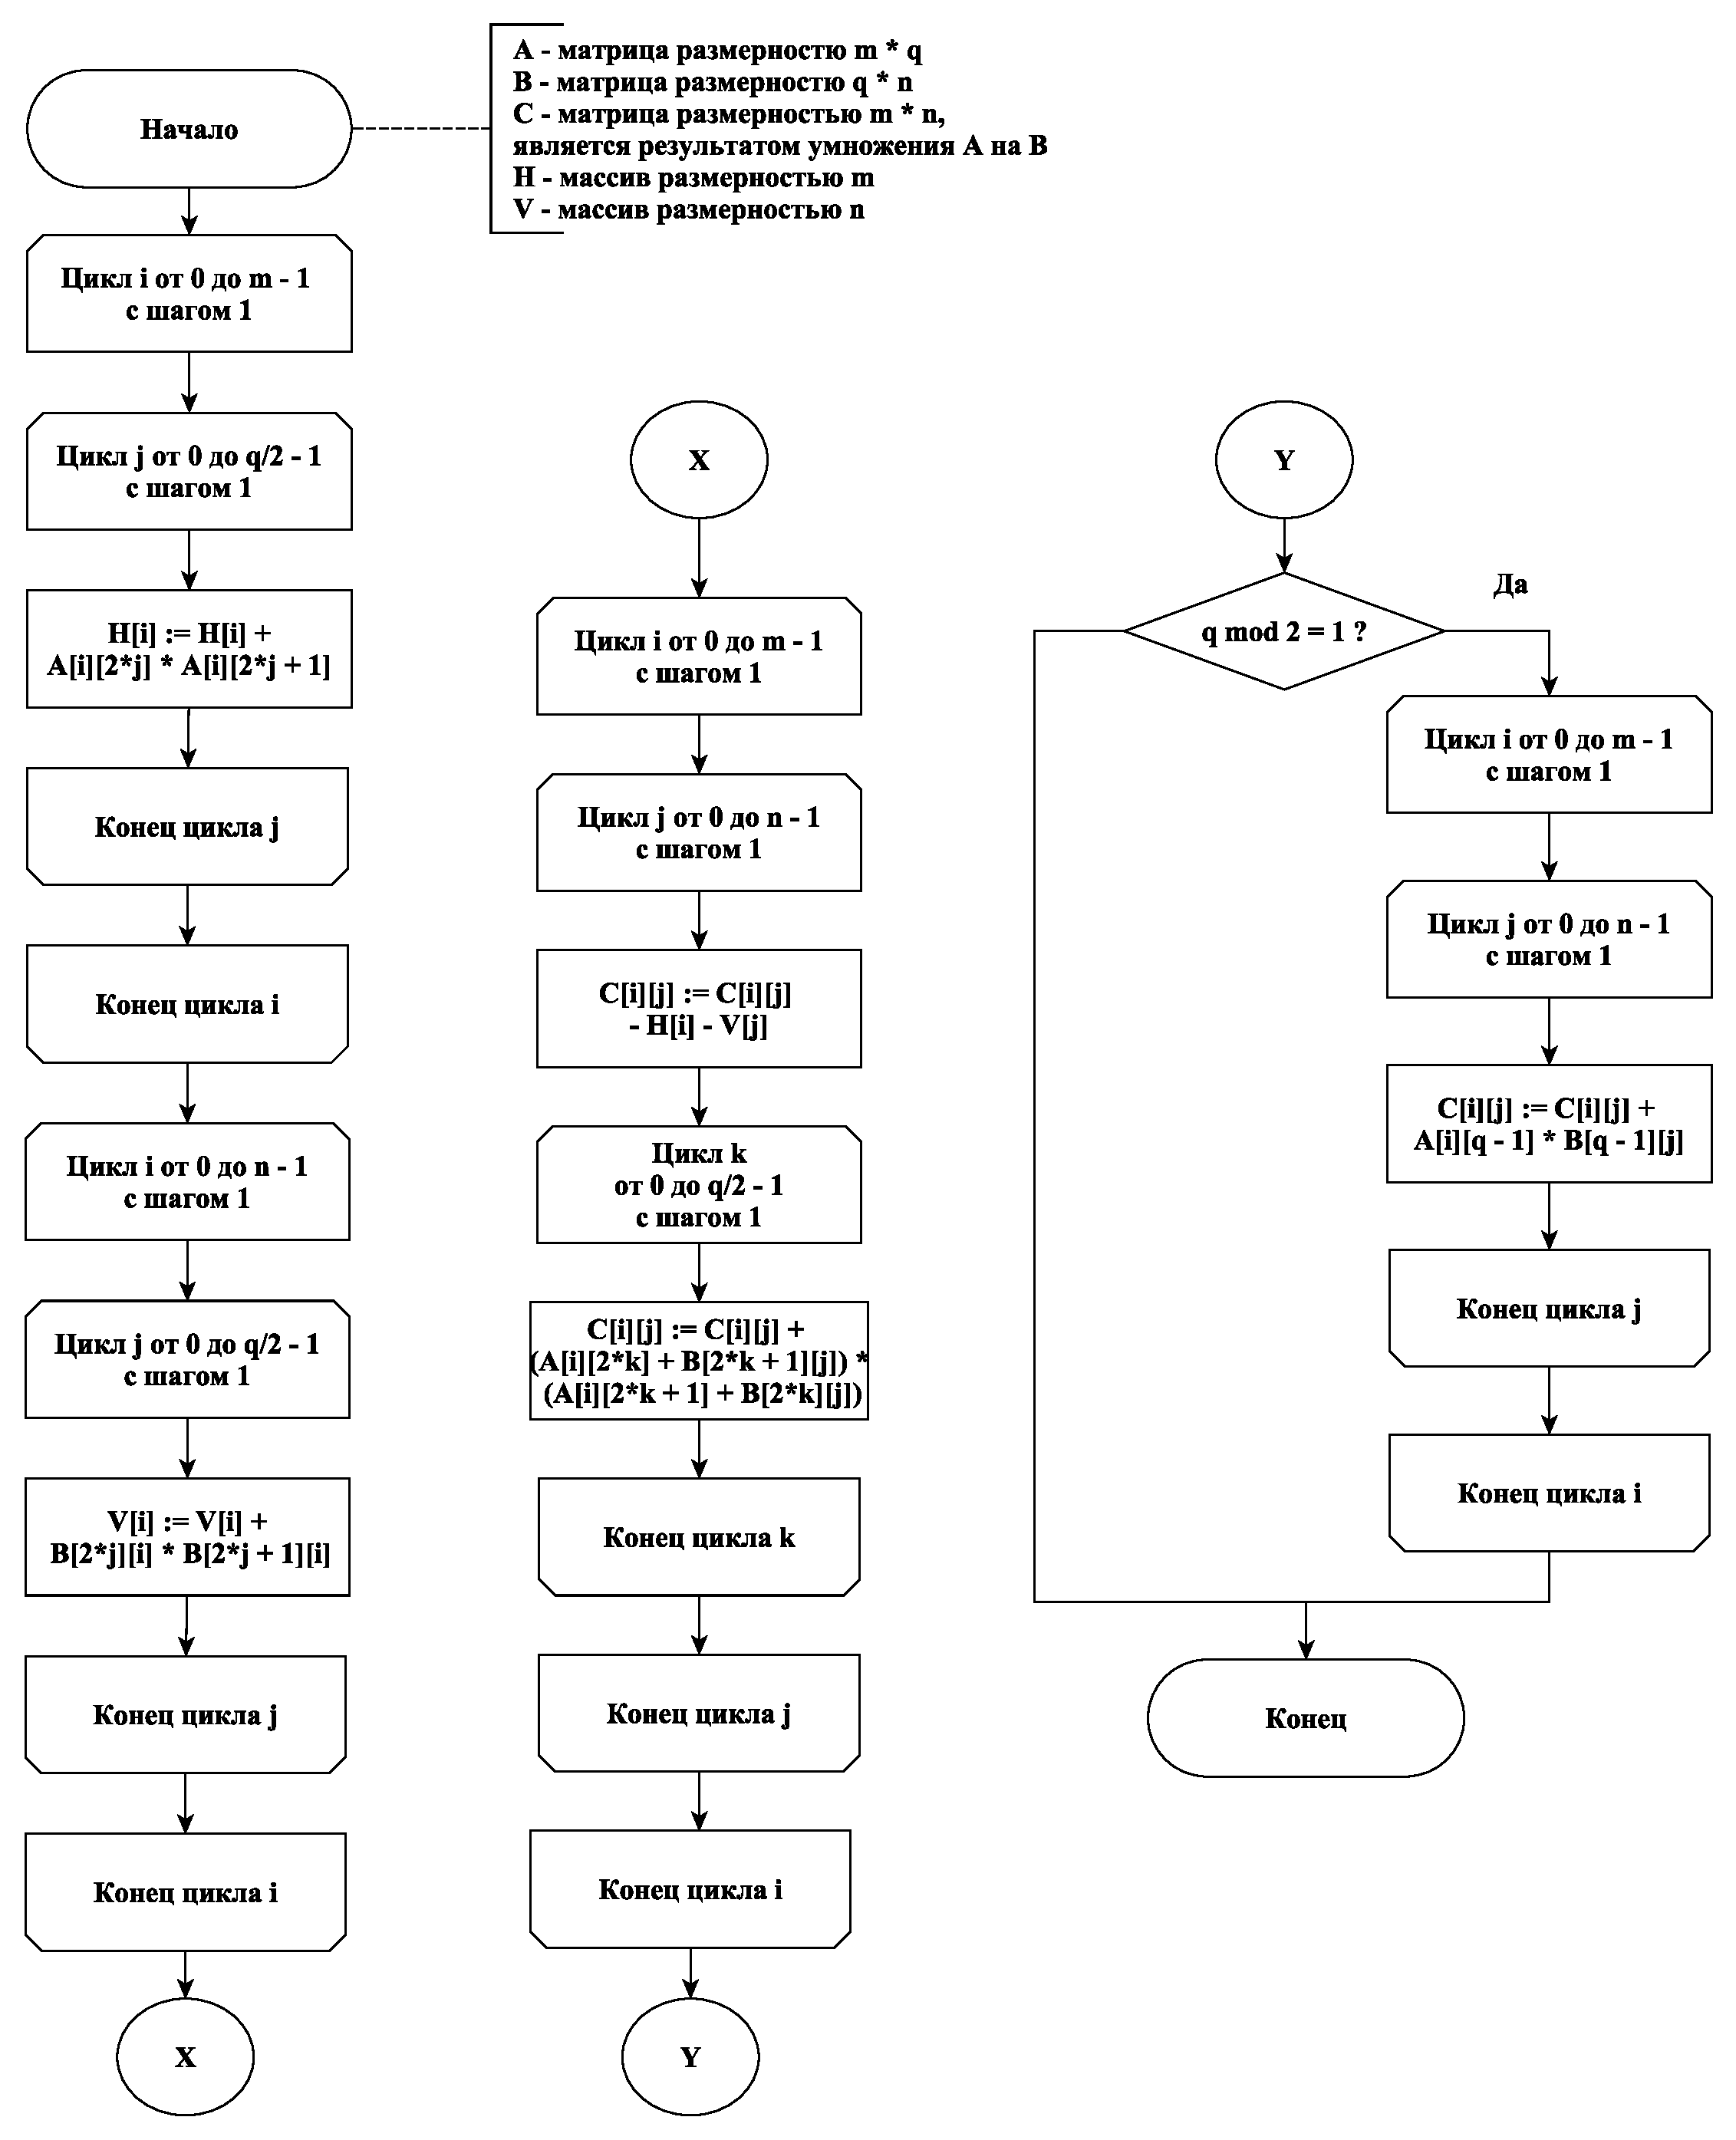
\includegraphics[width = \textwidth]{vinograd.pdf}}
		\caption{
			Умножение матриц по Винограду}
		\label{fig:vinograd}
	\end{center}
\end{figure}

На рис. \ref{fig:mod_vinograd} приведена схема оптимизированного
умножения матриц по Винограду.

\begin{figure}[h!]
	\begin{center}
		{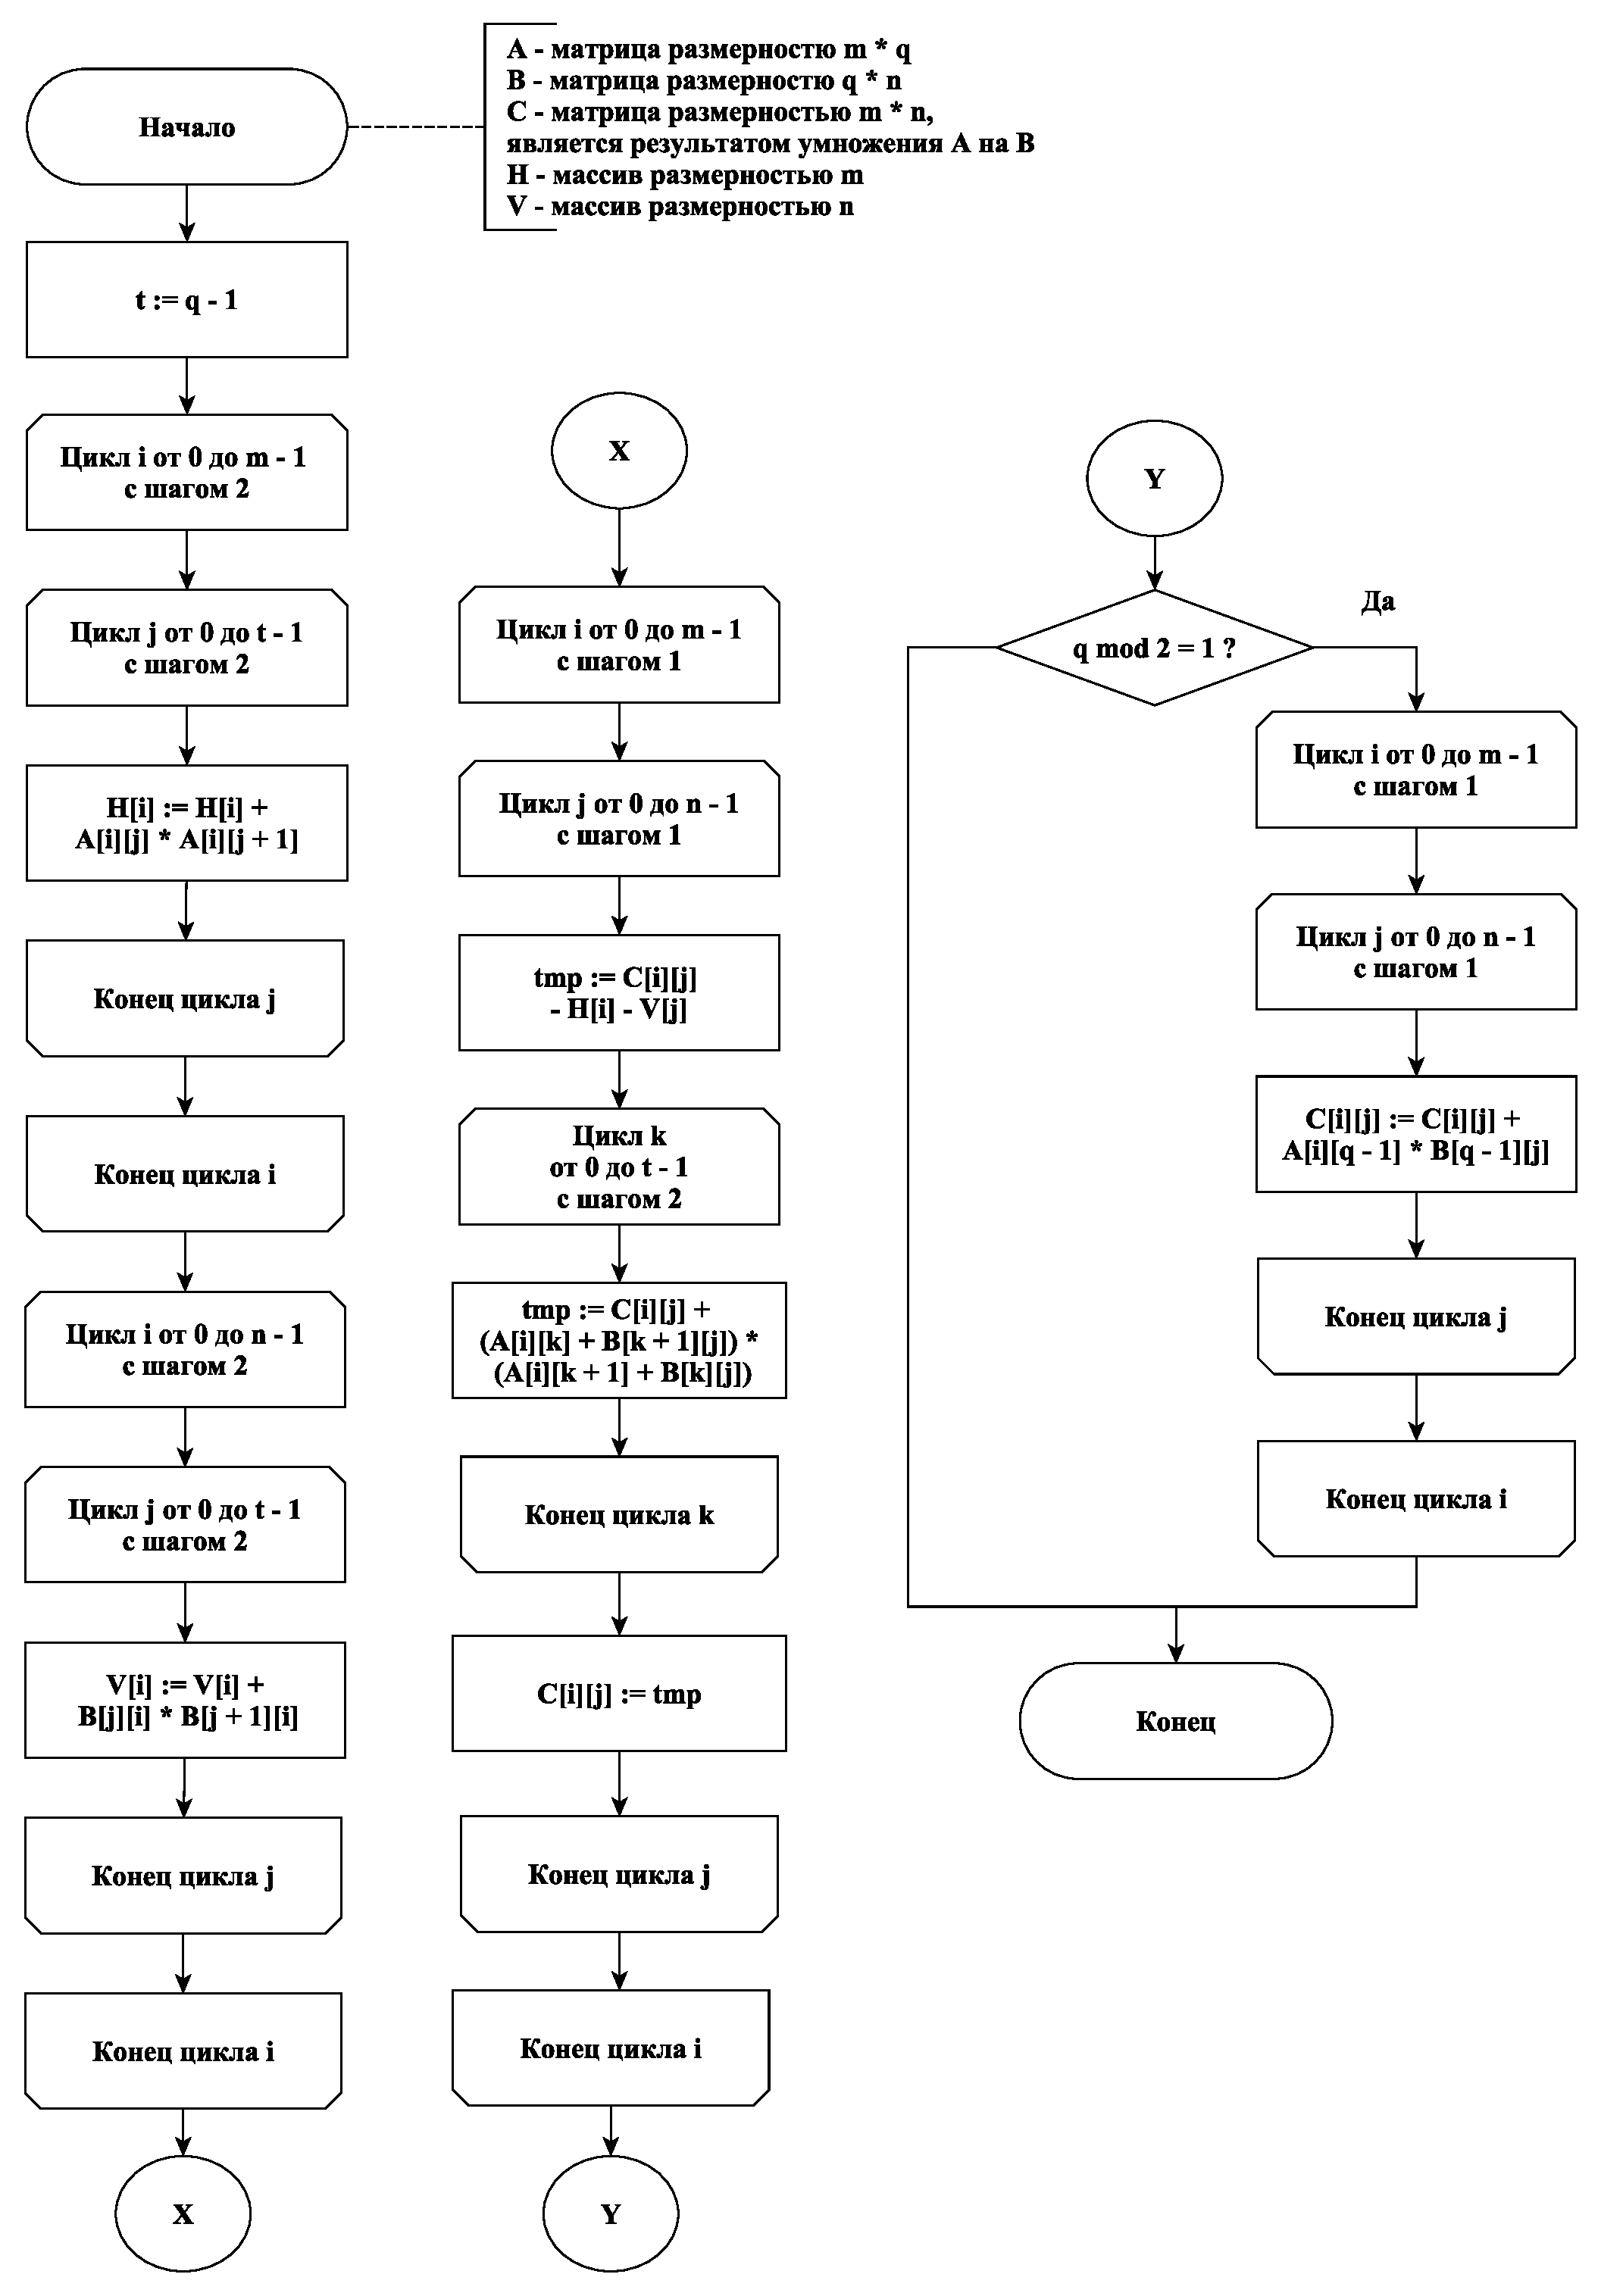
\includegraphics[scale = 0.48]
			{mod_vinograd.pdf}}
		\caption{
			Оптимизированное умножение матриц по Винограду}
		\label{fig:mod_vinograd}
	\end{center}
\end{figure}

\pagebreak

\subsection*{Выводы}
\addcontentsline{toc}{subsection}{Выводы}

В разделе представлены схемы стандартного алгоритма
умножения матриц,
обычного и оптимизированного алгоритмов Винограда.


\section{Технологический раздел}

Здесь описываются требования к программному 
обеспечению и средства реализации, приводится листинг 
программы и проводится сравнительный анализ 
потребления памяти.

\subsection{Требования к программному обеспечению}

\begin{flushleft}
	\textbf{Входные данные:} 
	\begin{itemize}
		\item количество используемых потоков,
		\item $m$ -- количество строк
		матрицы $\mathbf{A}$,
		\item $q$ -- количество столбцов
		матрицы $\mathbf{A}$ и строк матрицы $\mathbf{B}$,
		\item элементы матрицы $\mathbf{A}$,
		\item $n$ -- количество столбцов матрицы $\mathbf{B}$,
		\item элементы матрицы $\mathbf{B}$.
	\end{itemize}
	
	\textbf{Выходные данные:} матрица $\mathbf{C}$ 
	размерностью
	$m \times n$ -- результат умножения $\mathbf{A}$
	на $\mathbf{B}$, время выполнения в наносекундах.
\end{flushleft}

\subsection{Средства реализации}

Для реализации поставленной задачи был использован язык программирования C++ ~\cite{c}. Проект был выполнен в среде QT Creator ~\cite{qt}. Для измерения процессроного времени была использована ассемблерная инструкция rdtsc ~\cite{rdtsc}.

\subsection{Листинг программы}

Реализованная программа представлена
в листингах \ref{lst1}, \ref{lst2}, \ref{lst3} и \ref{lst4}.

\begin{lstlisting}[label=lst1, caption=Реализация оптимизированного алгоритма умножения матриц по Винограду]
Matrix modified_vinograd_mult(const Matrix &a, const Matrix &b) {
if (a.empty() || b.empty() || a[0].size() != b.size()) {
return Matrix();
}

size_t m = a.size();
size_t q = b.size();
size_t n = b[0].size();
Matrix c(m, std::vector<int>(n, 0));

size_t t = q - 1;
std::vector<int> row_fact(m, 0);
std::vector<int> col_fact(n, 0);

for (size_t i = 0; i < m; i++) {
for (size_t j = 0; j < t; j += 2) {
row_fact[i] += a[i][j] * a[i][j+1];
}
}

for (size_t i = 0; i < n; i++) {
for (size_t j = 0; j < t; j += 2) {
col_fact[i] += b[j][i] * b[j+1][i];
}
}

int tmp = 0;

for (size_t i = 0; i < m; i++) {
for (size_t j = 0; j < n; j++) {
tmp = -row_fact[i] - col_fact[j];
for (size_t k = 0; k < t; k += 2) {
tmp += (a[i][k] + b[k+1][j]) * (a[i][k+1] + b[k][j]);
}

c[i][j] = tmp;
}
}

if (q % 2) {
for (size_t i = 0; i < m; i++) {
for (size_t j = 0; j < n; j++) {
c[i][j] += a[i][q-1] * b[q-1][j];
}
}
}

return c;
}
\end{lstlisting}

\begin{lstlisting}[label=lst2,caption=Реализация
оптимизированного многопоточного алгоритма умножения матриц по Винограду]
void calc_row_fact(vector<int> &row_fact, size_t m, size_t t, const Matrix &a)
{
for (size_t i = 0; i < m; i++)
{
for (size_t j = 0; j < t; j += 2)
{
row_fact[i] += a[i][j] * a[i][j + 1];
}
}
}

void calc_col_fact(vector<int> &col_fact, size_t n, size_t t, const Matrix &b)
{
for (size_t i = 0; i < n; i++) {
for (size_t j = 0; j < t; j += 2) {
col_fact[i] += b[j][i] * b[j+1][i];
}
}
}

void par_calculations(size_t m, size_t n, size_t t, const Matrix &a,
const Matrix &b, Matrix &c, size_t thread,
size_t count_threads, const vector<int> &row_fact, const vector<int> &col_fact, int tmp)
{

for (size_t i = thread; i < m; i += count_threads) {
for (size_t j = 0; j < n; j++) {
tmp = -row_fact[i] - col_fact[j];
for (size_t k = 0; k < t; k += 2) {
tmp += (a[i][k] + b[k + 1][j]) * (a[i][k + 1] + b[k][j]);
}
c[i][j] = tmp;
}
}
}

void calc_dop_calculations(size_t m, size_t n, size_t q, const Matrix &a, const Matrix &b, Matrix &c, size_t thread, size_t count_theads)
{
for (size_t i = thread; i < m; i += count_theads)
{
for (size_t j = 0; j < n; j++)
{
c[i][j] += a[i][q - 1] * b[q - 1][j];
}
}
}

Matrix modified_thread_vinograd_mult(const Matrix &a, const Matrix &b, size_t count_threads)
{
if (a.empty() || b.empty() || a[0].size() != b.size()) {
return Matrix();
}

size_t m = a.size();
size_t q = b.size();
size_t n = b[0].size();
Matrix c(m, std::vector<int>(n, 0));

size_t t = q - 1;
std::vector<int> row_fact(m, 0);
std::vector<int> col_fact(n, 0);

thread row(calc_row_fact, ref(row_fact), m, t, ref(a));
thread col(calc_col_fact, ref(col_fact), n, t, ref(b));

row.join();
col.join();



vector<thread> threads(count_threads);

int tmp = 0;

for (size_t i = 0; i < count_threads; i++)
{
threads[i] = thread(par_calculations, m, n, t, ref(a), ref(b), ref(c), i, count_threads, ref(row_fact), ref(col_fact), tmp);
}

for (size_t i = 0; i < count_threads; i++)
{
threads[i].join();
}

if (q % 2)
{
for (size_t i = 0; i < count_threads; i++)
{
threads[i] = thread(calc_dop_calculations, m, n, q, ref(a), ref(b), ref(c), i, count_threads);
}

for (size_t i = 0; i < count_threads; i++)
{
threads[i].join();
}
}

return c;
}
\end{lstlisting}

\begin{lstlisting}[label=lst3,caption=Замер времени]
long long get_dif_threads(long long i1, long long i2, const Matrix &m1, const Matrix &m2, size_t count_threads)
{
i1  = __rdtsc();
Matrix m4 = modified_thread_vinograd_mult(m1, m2, count_threads);
i2  = __rdtsc();

return abs(i2 - i1);
}
} 
\end{lstlisting}

\subsection{Тестовые данные}
\label{fig:test_data}

Программа должна корректно работать при следующих 
входных данных:
\\
\begin{itemize}
	\item умножение матриц, состоящих из одного элемента:
	\[ \begin{pmatrix}
	2
	\end{pmatrix} \times 
	\begin{pmatrix}
	5
	\end{pmatrix} =
	\begin{pmatrix}
	10
	\end{pmatrix}, \]
	
	\item умножение на нулевую матрицу:
	\[ \begin{pmatrix}
	1 & -2 \\
	3 & -4
	\end{pmatrix} \times 
	\begin{pmatrix}
	0 & 0 \\
	0 & 0
	\end{pmatrix} =
	\begin{pmatrix}
	0 & 0 \\
	0 & 0
	\end{pmatrix}, \]
	
	\item умножение на единичную матрицу:
	\[ \begin{pmatrix}
	1 & -2 \\
	3 & -4
	\end{pmatrix} \times 
	\begin{pmatrix}
	1 & 0 \\
	0 & 1
	\end{pmatrix} =
	\begin{pmatrix}
	1 & -2 \\
	3 & -4
	\end{pmatrix}, \]
	
	\item умножение матриц с положительными числами:
	\[ \begin{pmatrix}
	1 & 2 \\
	3 & 4
	\end{pmatrix} \times 
	\begin{pmatrix}
	1 & 2 \\
	3 & 4
	\end{pmatrix} =
	\begin{pmatrix}
	7 & 10 \\
	15 & 22
	\end{pmatrix}, \]
	
	\item умножение матриц с отрицательными числами:
	\[ \begin{pmatrix}
	-1 & -2 \\
	-3 & -4
	\end{pmatrix} \times 
	\begin{pmatrix}
	-1 & -2 \\
	-3 & -4
	\end{pmatrix} =
	\begin{pmatrix}
	7 & 10 \\
	15 & 22
	\end{pmatrix}, \]
	
	\item умножение матриц нечетной размерности
	(актуально для алгоритма Винограда, т.к.
	используется дополнительная проверка):
	\[ \begin{pmatrix}
	1 & -2 & -3 \\
	-4 & 5 & 6 \\
	-7 & -8 & 9 
	\end{pmatrix} \times 
	\begin{pmatrix}
	-1 & 2 & -3 \\
	-4 & 5 & -6 \\
	-7 & 8 & -9 
	\end{pmatrix} =
	\begin{pmatrix}
	28 & -32 &  36 \\
	26 & -31 &  36 \\
	-24 & 18 & -12
	\end{pmatrix}, \]
	
	\item умножение матриц с целыми числами:
	\[ \begin{pmatrix}
	1 & -2 \\
	3 & -4
	\end{pmatrix} \times 
	\begin{pmatrix}
	-1 & 2 \\
	3 & -4
	\end{pmatrix} =
	\begin{pmatrix}
	-7 & 10 \\
	-15 & 22
	\end{pmatrix}, \]
	
	\item умножение прямоугольных матриц:
	\[ \begin{pmatrix}
	1 & -2 \\
	3 & -4 \\
	5 & -6 \\
	7 & -8
	\end{pmatrix} \times 
	\begin{pmatrix}
	10 & 100 & 1000 \\
	20 & 200 & 2000
	\end{pmatrix} =
	\begin{pmatrix}
	-30 & -300 & -3000 \\
	-50 & -500 & -5000 \\
	-70 & -700 & -7000 \\
	-90 & -900 & -9000
	\end{pmatrix}. \]
	
\end{itemize}

\subsection{Сравнительный анализ реализаций}
\label{fig:cmp}

Примем следующую теоретическую модель вычислений для
оценки трудоемкости алгоритмов:

\begin{enumerate}
	\item[1)] операции единичной стоимости (арифметические, сравнения, обращение по адресу);
	\item[2)] циклы определяются формулой:
	\begin{multline}
		f_{cycle} = f_{init} + f_{cmp} + n \cdot (f_{inner} + f_{inc} + f_{cmp}) = \\
		= 1 + 1 + n \cdot (f_{inner} + 1 + 1) = \\
		= 2 + n \cdot (f_{inner} + 2),
	\end{multline}
	\begin{flushleft}
		где \\
		$n$ --- количество итераций цикла,\\ 
		$f_{cycle}$ --- трудоемкость цикла,\\
		$f_{init}$ --- трудоемкость инициализации,\\
		$f_{cmp}$ --- трудоемкость сравнения,\\
		$f_{inner}$ --- трудоемкость тела цикла,\\
		$f_{inc}$ --- трудоемкость инкремента;\\
	\end{flushleft}
	
	\item[3)] переход по условию в условном операторе равен нулю, но при этом в расчет входит трудоемкость вычисления условия. 
\end{enumerate}

Пусть даны две матрицы $\mathbf{A}$ размерностью
$m \times q$ и $\mathbf{B}$ размерностью $q \times n$,
результат их умножения --- матрица $\mathbf{C}$
размерностью $m \times n$.

\subsubsection{Трудоемкость стандартного алгоритма}

Опираясь на указанные выше правила, подсчитаем трудоемкость стандартного алгоритма умножения матриц:
\begin{multline}
	f_{std} = 2 + m \cdot (2 + 2 + n \cdot
	(2 + 2 + q \cdot (2 + \underbrace{8}_{[\:]} +
	\underbrace{1}_{=} +
	\underbrace{1}_{+} + 
	\underbrace{1}_{\times}))) = \\
	= 13mqn + 4mn + 4m + 2
\end{multline}

\subsubsection{Трудоемкость алгоритма Винограда}

Заполнение массива под произведения строчных элементов:
\begin{multline}
	f_{row} = 2 + m \cdot(2 + 2 + 1 + \frac{q}{2} \cdot
	(3 + \underbrace{6}_{[\:]} +
	\underbrace{1}_{=} +
	\underbrace{2}_{+} +
	\underbrace{3}_{\times}
	)) = \\
	= \frac{15}{2}mq + 5m + 2.    
\end{multline}

Заполнение массива под произведения элементов столбцов производится аналогично, поэтому можно перейти сразу
к формуле:
\[
f_{col} = \frac{15}{2}qn + 5n + 2.    
\]

Основной цикл вычисления значений элементов
результирующей матрицы:
\begin{multline}
	f_{inner} = 2 + m \cdot 
	(2 + 2 + n \cdot
	(2 + 7 + 3 + \frac{q}{2} \cdot
	(3 + 
	\underbrace{12}_{[\:]} + 
	\underbrace{1}_{=} + 
	\underbrace{5}_{+} + 
	\underbrace{5}_{\times}
	))) = \\
	= 13mqn + 12qn + 4m + 2.
\end{multline}

Учет условия перехода при значении $q$:
\[
f_{cond} = 2 + 
\left [
\begin{aligned}
&0, если q - четное, \\
&2 + m \cdot (2 + 2 + n \cdot (2 + 
\underbrace{8}_{[\:]} + 
\underbrace{1}_{=} + 
\underbrace{1}_{+} + 
\underbrace{2}_{-} + 
\underbrace{1}_{\times}
)), иначе,
\end{aligned}
\right. = \\
= 2 + \left [
\begin{aligned}
&0, если q - четное, \\
&15mn + 4m + 2, иначе.
\end{aligned}
\right. 
\]

Таким образом, получаем формулу вычисления
произведения матриц алгоритмом Винограда:
\[
f_{V} = 
13mqn + \frac{15}{2}mq + \frac{39}{2}qn + 
9m + 5n + 8 + \left [ 
\begin{aligned}
&0, если q - четное, \\
&15mn + 4m + 2, иначе.
\end{aligned}
\right.
\]

\subsubsection{Трудоемкость 
	оптимизированного алгоритма Винограда}

Заполнение массива под произведения строчных элементов:
\begin{multline}
	f_{row} = 2 + m \cdot(2 + 2 + \frac{q}{2} \cdot
	(3 + \underbrace{5}_{[\:]} +
	\underbrace{1}_{+} +
	\underbrace{1}_{+=} +
	\underbrace{1}_{\times}
	)) = \\
	= \frac{11}{2}mq + 4m + 2.    
\end{multline}

Заполнение массива под произведения элементов столбцов производится аналогично, поэтому можно перейти сразу
к формуле:
\[
f_{col} = \frac{11}{2}qn + 4n + 2.    
\]

Основной цикл вычисления значений элементов
результирующей матрицы:
\begin{multline}
	f_{inner} = 2 + m \cdot 
	(2 + 2 + n \cdot
	(2 + 9 + 3 + \frac{q}{2} \cdot
	(3 + 
	\underbrace{8}_{[\:]} + 
	\underbrace{1}_{=} + 
	\underbrace{2}_{+} + 
	\underbrace{1}_{+=} + 
	\underbrace{1}_{\times}
	))) = \\
	= 8mqn + 14qn + 4m + 2.
\end{multline}

Учет условия перехода при значении $q$:
\[
f_{cond} = 1 + 
\left [
\begin{aligned}
&0, если q - четное, \\
&2 + m \cdot (2 + 2 + n \cdot (1 + 
\underbrace{6}_{[]} + 
\underbrace{1}_{+} + 
\underbrace{2}_{-} + 
\underbrace{1}_{\times}
)), иначе,
\end{aligned}
\right. = \\
= 2 + \left [
\begin{aligned}
&0, если q - четное, \\
&\frac{11}{2}mn + 4m + 2, иначе.
\end{aligned}
\right. 
\]

Конечная формула:
\[
f_{V} = 
8mqn + \frac{11}{2}mn + \frac{39}{2}qn + 
8m + 4n + 6 + \left [ 
\begin{aligned}
&0, если q - четное, \\
&\frac{11}{2}mn + 4m + 2, иначе.
\end{aligned}
\right.
\]


\subsection*{Выводы}
\addcontentsline{toc}{subsection}{Выводы}

В данном разделе были рассмотрены требования к 
программному обеспечению, обоснован выбор средств 
реализации, приведён листинг программы и тестовые 
данные.

\section{Исследовательский раздел}

В разделе представлены результаты тестирования, постановка и результаты экспериментов, а также их сравнительный анализ.

\subsection{Результаты тестирования}

Все тесты из раздела \ref{fig:test_data} 
успешно пройдены.

\subsection{Постановка эксперимента}

Необходимо cравнить время работы оптимизированного алгоритма Винограда и оптимизированного алгоритма Винограда на 1-ом, 2-мя, 4-мя, 8-ю и 32-мя рабочими потоками на квадратных матрицах $100 \times 100$.

\subsection{Сравнительный анализ на основе эксперимента}

Экспериментально получена таблица сравнения времени
\ref{restable}:

\newpage

\begin{table} [h!]
	\begin{center}
		\caption{Сравнение времени выполнения оптимизированного алгоритма Винограда и оптимизированного алгоритма Винограда на разных потоках на квадратных матрицах $100 \times 100$ в тиках}
		\begin{tabular}{|c|c|c|c|}
			\hline 
			Кол-во потоков & Размерность & Виноград (опт.) & Виноград (опт. + потоки)\\ 
			\hline 
			1 & 100 & 30350926 & 31278636 \\ 
			\hline 
			2 & 100 & 30350926 & 13545137 \\ 
			\hline 
			4 & 100 & 30350926 & 10040994 \\ 
			\hline
			8 & 100 & 30350926 & 8486562 \\ 
			\hline 
			16 & 100 & 30350926 & 8785022 \\ 
			\hline 
			32 & 100 & 30350926 & 8936443 \\ 
			\hline
		\end{tabular}
		\label{restable}
	\end{center}
\end{table}

На рис. \ref{fig:graph} приводятся графики сравнения времени выполнения выбранных алгоритмов.

\begin{tikzpicture}
\label{fig:graph}
\begin{axis}[
axis lines = left,
xlabel = {$count$, потоков},
ylabel = {$time$, тактов},
legend pos=north west,
ymajorgrids=true
]
\addplot[color=red] table[x index=0, y index=1] {Vinograddd.dat};
\addplot[color=green, mark=square] table[x index=0, y index=1] {Thread_vinograddd.dat};

\addlegendentry{Vinograd}
\addlegendentry{Thread\_vinograd}

\end{axis}
\end{tikzpicture}

Как видно, при 8-ми потоках достигается наибольшая производительность. При этом разница во времени выполнения алгоритмов Винограда и Винограда с потоками различается почти в 4 раза.

\subsection*{Выводы}
\addcontentsline{toc}{subsection}{Выводы}

Программа успешно прошла все заявленные тесты. Эксперименты замера времени  показали, что эффективнее всего использовать 8 рабочих потоков на алгоритме Винограда. При этом алгоритм Винограда на одном потоке работает почти в 4 раза медленней.


\section*{Заключение}
\addcontentsline{toc}{section}{Заключение}

В ходе работы выполнено следующее:

\begin{enumerate} 
	\item[1)] изучен алгоритм умножения матриц по Винограду;
	\item[2)] оптимизирован алгоритм Винограда;
	\item[3)] реализована многопоточность для оптимизированного алгоритма Винограда;
	\item[3)] применен метод динамического программирования для реализации указанных алгоритмов;
	\item[4)] проведен сравнительный анализ по затрачиваемому времени при разном количестве рабочих потоков;
	\item[5)] описаны и обоснованы полученные результаты в отчете, выполненного как расчётно-пояснительная записка к работе. 
\end{enumerate}

Эксперименты замера времени показали, что при последовательной и параллельной (с одним рабочим потоком) реализациях оптимизированного алгоритма Винограда совсем немного выигрывает последовательная реализация (в ней не тратится время на выделение рабочего потока). На матрицах размером $100 \times 100$ последовательная реализация на 0.0015\% быстрее параллельной.

При сравнении замеров времени для параллельной реализации алгоритма с 1-м, 2-мя, 4-мя, 8-ю, 16-ю и 32-мя рабочими потоками выяснилось, что максимальная производительность достигается на 8-ми рабочих потоках , что равно количеству логических потоков компьютера, на котором производились замеры. Выполнение алгоритма на 8-ми рабочих потоках быстрее в 3,95 раз, по сравнению с выполнением на 1-м потоке для матриц размера $100 \times 100$. При большем количестве рабочих потоков происходит небольшое падение производительности (тратится время на создание новых рабочих потоков, но вычисления будут производиться с той же скоростью, что и при 8 рабочих потоках).

\pagebreak

\addcontentsline{toc}{section}{Список литературы}
\begin{thebibliography}{}
	
	\bibitem{mcconell}
	Дж. Макконнелл. Анализ алгоритмов. Активный 
	обучающий 
	подход.-М.:Техносфера, 2009.
	
	\bibitem{bioinf}
	Group-theoretic Algorithms for Matrix Multiplication
	[Электронный ресурс]. – Режим доступа: http://users.cms.caltech.edu/~umans/papers/CKSU05.pdf, свободный – 
	(10.10.2019)
	
	\bibitem{bioinf}
	Уменьшена экспонента умножения матриц
	[Электронный ресурс]. – Режим доступа: 
	https://habr.com/ru/post/133875/, свободный – 
	(11.10.2019)
	
	\bibitem{latex_book}
	Библиография в LaTeX [Электронный ресурс]. – Режим 
	доступа: https://habr.com/ru/post/114997/, свободный 
	– (26.09.2019)
	
	\bibitem{qt} QT Creator Manual [Электронный ресурс]. – Режим
	доступа: https://doc.qt.io/qtcreator/index.html, свободный. (Дата
	обращения: 29.09.2019 г.)
	
	\bibitem{rdtsc} Microsoft «rdtsc» [Электронный ресурс]. – Режим доступа:
	https://docs.microsoft.com/ru-ru/cpp/intrinsics/rdtsc?view=vs-2019,
	свободный. (Дата обращения: 29.09.2019 г.)
	
	\bibitem{c} ISO/IEC JTC1 SC22 WG21 N 3690 «Programming Languages — C++» [Электронный ресурс]. – Режим доступа: https://devdocs.io/cpp/, свободный. (Дата обращения: 29.09.2019 г.)
	
\end{thebibliography}



\end{document}